\begin{figure}[h]\begin{center}
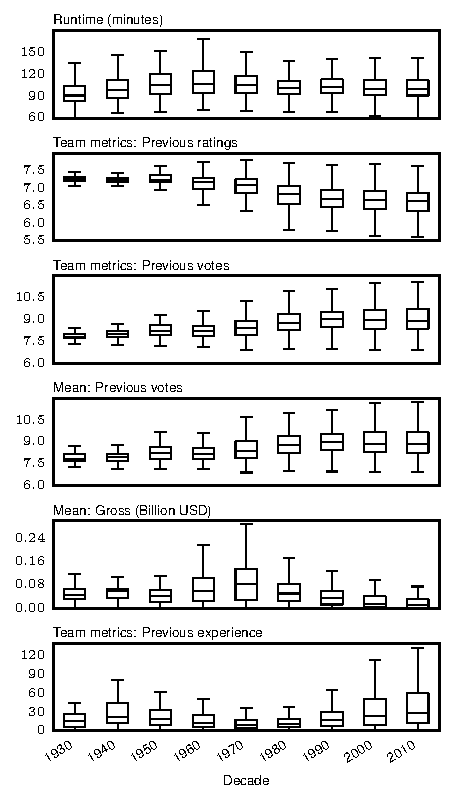
\includegraphics[width=0.7\columnwidth,height=18cm]{../../images/features_dist_ntop.pdf}
\caption{\label{fig:features_dist_ntop}Distribution of non-topological features
throughout the years.}
\end{center}\end{figure}

\section{Feature Characterization}
\label{sec:feature_char}
We present distributions from the selected features across the decades in
Figures~\ref{fig:features_dist_ntop}~and~\ref{fig:features_dist_top}. Features
have very different distributions throughout the years, indicating that the
movie producing network is dynamic and constantly evolving, albeit in a slow
pace\footnote{Figures~\ref{fig:hist_feat_ntop}~and~\ref{fig:hist_feat_top}
(presented in detail in Chapter~\ref{chapter:analysis}) present the
distribution of selected features in the whole set of data, but in the form of
color-coded histogram bars according to the movies performance group.}

\begin{figure}[!htb]\begin{center}
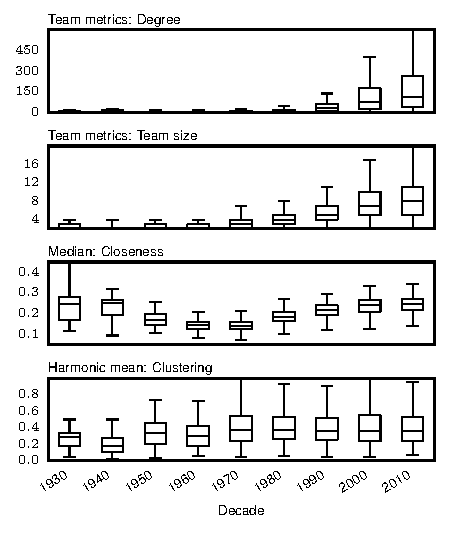
\includegraphics[width=0.78\columnwidth]{../../images/features_dist_top.pdf}
\caption{\label{fig:features_dist_top}Distribution of topological features
throughout the years.}
\end{center}\end{figure}

\begin{figure}[!htb]\begin{center}
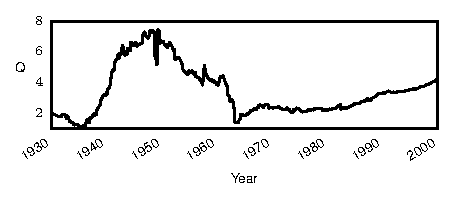
\includegraphics[width=0.78\columnwidth]{../../images/plot_q_1k.pdf}
\caption{\label{fig:q}Evolution of the small world coefficient for the IMDb network
cut considered in this research.}
\end{center}\end{figure}

We can see from these characterizations that different performance groups have
different distributions for the features being extracted. This is an important
indicator that the extracted features can indeed provide information on movie
performance.

Analyzing the features and their distributions also yields interesting insights
into the network. Figure~\ref{fig:q} shows the evolution of the small world
coefficient from the whole graph thorough the years. We can see a clear
disruption in the organization of the network in the 40s and 50s, that was
probably caused by World War II.\@ The efforts on the war and infrastructural
recovery that followed it could have captured resources that were previously
available for movie production. Also, the war destruction could have taken away
many filming sets, equipments, and even lives of actors and producers.

We observe that the post-war rise in the network's small world coefficient was
not as intense as in pre-war years. We hypothesise that this reflects a greater
division of the world, as movies producers from opposing cold war countries
would not be able to cooperate. Also, during the Cold War, producers and
directors (mostly in the USA) were persecuted as communists, that lead to a
decrease in production. Moreover, in recent years the cost of movie
production went down, what could have resulted in a greater pool of movie
producers spread around the world, leading to the existence of more teams that
are not closely knit in a central core.
